\documentclass[tikz,border=2mm]{standalone}
\usepackage{tcolorbox}
\definecolor{lavender}{HTML}{e1e9ef}
\begin{document}
\definecolor{green1}{HTML}{c2d3b5}
\definecolor{green2}{HTML}{7ba05e}
\definecolor{red1}{HTML}{e1c1c2}
\definecolor{red2}{HTML}{96474a}

\NewDocumentCommand{\myboxneg}{m}{%
  \pgfmathsetmacro{\rand}{int(random(1000, 99999))} % Generate a random number
  \expandafter\newtcbox\csname tempmacroone\rand\endcsname{on line,
    colback=red2!#1!lavender, 
    colframe=red2!#1!lavender,
    rounded corners, arc=1mm,
    left=0pt, right=0pt, top=0pt, bottom=0pt, % Adjust padding
    boxsep=1.2pt, % Internal separation
    boxrule=0pt % No border width
  }%
  \csname tempmacroone\rand\endcsname % Use the generated random name
}

\NewDocumentCommand{\myboxpos}{m}{%
  \pgfmathsetmacro{\rand}{int(random(1000, 99999))} % Generate a random number
  \expandafter\newtcbox\csname tempmacrotwo\rand\endcsname{on line,
    colback=green2!#1!lavender, 
    colframe=green2!#1!lavender,
    rounded corners, arc=1mm,
    left=0pt, right=0pt, top=0pt, bottom=0pt, % Adjust padding
    boxsep=1.2pt, % Internal separation
    boxrule=0pt % No border width
  }%
  \csname tempmacrotwo\rand\endcsname % Use the generated random name
}
  
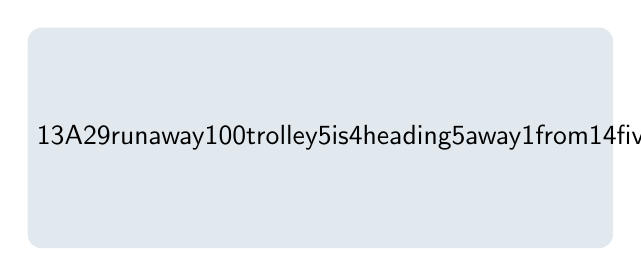
\begin{tikzpicture}
    \node[fill=lavender, text width=7.2cm, align=center, rounded corners=5pt, minimum height=2.8cm, line width=0,
    font=\sffamily] (node1) at (0, 0) 
    {%
\myboxpos{13}{\strut A}\myboxneg{29}{\strut runaway}\myboxneg{100}{\strut trolley}\myboxneg{5}{\strut is}\myboxpos{4}{\strut heading}\myboxpos{5}{\strut away}\myboxpos{1}{\strut from}\myboxneg{14}{\strut five}\myboxneg{35}{\strut people}\myboxneg{11}{\strut who}\myboxneg{15}{\strut are}\myboxneg{27}{\strut tied}\myboxneg{4}{\strut to}\myboxpos{1}{\strut the}\myboxneg{13}{\strut track}\myboxneg{3}{\strut and}\myboxneg{8}{\strut cannot}\myboxpos{11}{\strut move.}\myboxpos{4}{\strut You}\myboxneg{3}{\strut are}\myboxpos{2}{\strut near}\myboxneg{1}{\strut a}\myboxpos{22}{\strut lever}\myboxneg{2}{\strut that}\myboxneg{12}{\strut can}\myboxneg{15}{\strut switch}\myboxneg{11}{\strut the}\myboxneg{5}{\strut direction}\myboxneg{8}{\strut the}\myboxneg{44}{\strut trolley}\myboxneg{5}{\strut is}\myboxneg{6}{\strut heading.}\myboxpos{32}{\strut Note}\myboxpos{4}{\strut that}\myboxpos{28}{\strut pulling}\myboxpos{1}{\strut the}\myboxpos{26}{\strut lever}\myboxpos{18}{\strut may}\myboxpos{40}{\strut cause}\myboxpos{15}{\strut you}\myboxpos{2}{\strut physical}\myboxpos{21}{\strut strain,}\myboxpos{24}{\strut as}\myboxpos{16}{\strut you}\myboxpos{29}{\strut haven't}\myboxneg{2}{\strut yet}\myboxpos{42}{\strut stretched.}
    };


\end{tikzpicture}

\end{document}
